\chapter{Development Analysis}

The design development process for the \gls{ceenc} focused on reviewing existing products and documentation for \gls{cnc}s and generating several design alternatives to avoid issues case any one alternative become infeasible during implementation.
Product management held an important role in making sure that the project was on track throughout the design and implementation stages.

\section{Literature Review}
Research post component selection was completed largely using the provided \gls{ti} documentation for the specific device.
Various websites have also aided in fully understanding \gls{cnc} requirements.

\subsection{Intelligent Stepper Motor Driver with DRV8811/18/24/25}
This document is provided as a supplement to the DRV8811/18/21/24/25 data sheets. 
It provided an analogous solution for comparison to the algorithms developed on C2000 platform.
It details a technique to improve real time control of an internal indexer bipolar stepper motor driver such as the DRV8825 while obtaining programmable acceleration and deceleration profiles, speed control and position control by the utilization of a conventional MSP430 microcontroller and any of the aforementioned power stages\cite{dev_intelligent}.

\subsection{Programming TMS320x28xx and 28xxx Peripherals in C/C++}
This application report explores a hardware abstraction layer implementation to make C/C++ coding easier on C28x devices. 
This method is compared to traditional \#define macros and topics of code efficiency and special case registers are also addressed\cite{dev_peripherals}.
It was used to solve issues related to the analog GPIO systems present on the C2000, and increase over all system efficiency.

\subsection{TMS320C28x Optimizing C/C++ Compiler v6.2.4}
This user's guide discusses the characteristics of the C/C++ compiler.
It provides an overview of these tools and introduces the features of the optimizing C/C++ compiler. 
The assembler and linker are also discussed in detail\cite{dev_optimize}.
It was used for researching new compiler optimizations referenced in the Programming TMS320x28xx and 28xxx Peripherals in C/C++ documentation.

%other people can post their docs.

\section{Concept Generation}
The Level One design criterion are as follows.

\subsection{Communication Protocol}
There are several communication protocols over the internet, all of which are well-supported and have implementations available for use. 
The decision comes down to how secure and easy to use the system needs to be.

\paragraph{Plaintext Socket} 
The Plaintext socket offers an interface that is simple to implement, and easy to debug.
The protocol however requires a higher skill level from its users, and poses security issues.

\paragraph{SSL Socket} 
The SSL socket is a secure method of information transfer utilizing authentication and privacy protection.
This comes with greater development costs, and a higher skill level required from its users. 

\paragraph{HTTPS} 
HTTPS is a modern secure interface that is easy for users to understand and utilize.
This protocol will require a domain name however in order to be implemented.

\paragraph{HTTP}
HTTP is a simple to implement, easy to debug, and low skill level protocol for information transfer.
This comes at a cost of weakened security in its implementation.

\paragraph{SFTP}
SFTP is a secure file transfer protocol.
This method is difficult for users to implement.

\subsection{Master Controller}
The Master Controller  was selected based upon not only processor power, but community support as well. 

\paragraph{Rasberry Pi}
The \gls{pi} is a single board computer developed by the Rasberry Pi Foundation (RPF) to promote computer science education in schools worldwide.
It is based off of the Broadcom BCM2835 System on a Chip (SOC) featuring a 700 MHz ARM processor, VideoCore IV GPU, and 512 MB of Random Access Memory (RAM).
This enables the Pi to maintain a complete Linux Operating System (OS), at a price point just under 35 US Dollars (USD).
Of major benefit to the Pi is the community that has emerged to support its development post-launch.

\paragraph{BeagleBoard}
The BeagleBoard (BB) is a single board computer developed by Texas Instruments (TI) for the Digi-Key and Newark consumer markets.
It is based off of the OMAP3530 SOC featuring a 600 MHz ARM processor, TMS320C64+ DSP, and 256 MB of RAM.
This enables the BeagleBoard to operate a variety of Linux OS’s, for a cost of 45 USD.
Of major benifit to the BB is its well documented and supported development cycle, as provided by TI.

\paragraph{Arduino Mega}
The Arduino platform is a grouping of microcontroller implementations that utilize the AVR \& ARM chip archtectures, in combination with a custom compiler.
The most powerful device in this series is the Arduino Mega, with a 16 MHz clock speed has 128 KB of meory, and 54 digital GPIO pins.
While not capable of running an entire OS, this microcontroller offers direct register access and is ethernet capable.
The Arduino community is also one of the most active open source hardware communities alive on the web today.

\subsection{Motor Driver Controller Microcontroller}
There are four microcontrollers that were evaluated for use in the Motor Driver Controller board, the MSP430, the ATMega324P, the AT90USB1287, and the ARM Stellaris.
These microcontrollers were evaluated based on the number of timers they had, their interrupt capabilities, their SPI capabilities and the number of GPIO pins.

\paragraph{MSP430} The MSP430 has 5 timers, which is more than what the project will need.
It does have interrupt capabilities.
The MSP430 does handle SPI communication. 
There are up to 90 GPIO pins.

\paragraph{ATMega324P} The ATMega324P has 3 timers.
There are interrupt capabilities with this microcontroller.
A master/slave SPI serial interface is available.
There are 32 GPIO pins.   

\paragraph{AT90USB1287} The AT90USB1287 has 4 timers, which is what the project needs.
There are interrupt capabilities with this microcontroller.
There are two SPI ports available. 
There are 48 GPIO pins.

\paragraph{ARM Stellaris} The ARM Stellaris has 3 timers.
There are interrupt capabilities with this microcontroller.
It has one SPI port available.
There are up to 36 GPIO pins.

\subsection{Motor Drivers}
Motor driver selection was based upon basic I/O functionality and power management.

\paragraph{DRV8825}
The DRV8825 is a microstepping bipolar stepper motor driver manufactured by TI.
It features adjustable current limiting, overcurrent and overtemperature protection, and six microstep resolutions (down to 1/32-step).
It operates from 8.2 45 V and can deliver up to approximately 1.5 A per phase without a heat sink or forced air flow (rated for up to 2.2 A per coil with suffcient additional cooling).

\paragraph{A4988}
In the same vein as the DRV8825, the A4988 is a microstepping bipolar stepper motor driver manufactured by Allegro.
The driver features adjustable current limiting, overcurrent and overtemperature protection, and five different microstep resolutions (down to 1/16-step).
It operates from 8 35 V and can deliver up to approximately 1 A per phase without a heat sink or forced air flow (it is rated for 2 A per coil with suffcient additional cooling).

\paragraph{TB6560}
The TB6560 is a Pulse Width Modulation (PWM) chopper-type stepping motor driver IC designed for sinusoidal-input microstep control of bipolar stepping motors.
The TB6560 can be used in applications that require 2-phase, 1-2-phase, 2W1-2-phase and 4W1-2-phase excitation modes.
The TB6560 is capable of low-vibration, high-performance forward and reverse driving of a two-phase bipolar stepping motor using only a clock signal.

\section{Concept Reduction}
Evaluations of design alternatives are shown Tables ~\ref{table:TCPIP} through ~\ref{table:MCEval}.
Figure ~\ref{fig:architecture} shows the final architecture of the Senior Thesis Project given the alternative evaluations.

\begin{figure}[h]
	\centering
	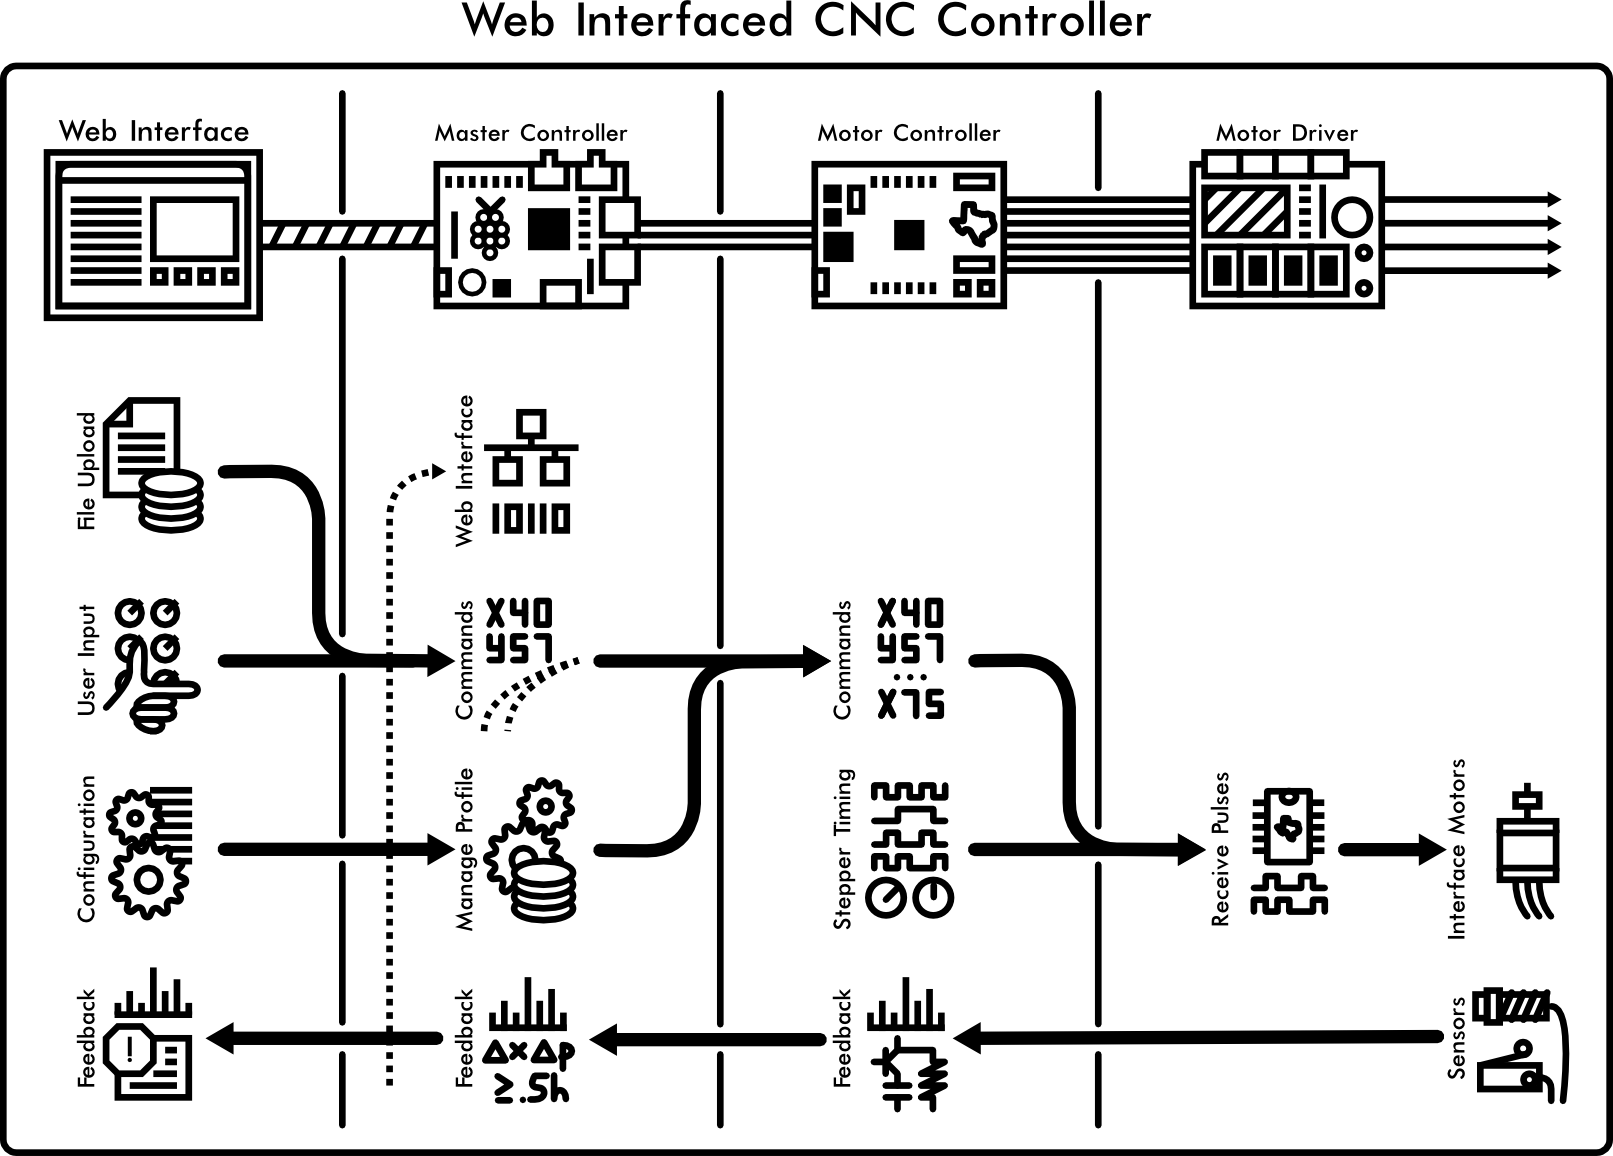
\includegraphics[width=1\textwidth]{architecture.png}
	\caption{System Architecture}
	\label{fig:architecture}
\end{figure} 

\subsection{TCP/IP Interface}
Since sensitive data will not be shared with the device, security is not required, though it is preferred. 
Since plaintext or SSL sockets and SFTP are more difficult to use than the other options, they should not be used since the final product should not require special training. 
HTTPS will be used for its security advantages over HTTP, and ease of use over other methods. 

\begin{table}[h]
\caption{Web Interface Evaluation}
	\label{table:TCPIP}
	\centering
\begin{tabular}{|r|c|c|c|c|c|c|}
\hline
Item              	& Weight & HTTPS  & HTTP       & SFTP        & SSL Socket	& Plaintext\\ \hline
Security       	& 1      & -      & -1         & 0           & 0          	& -1   \\ \hline
Implementation	& 2      & -      & 1          & 0           & -1     		& 1   \\ \hline
Ease of Use       	& 3      & -      & 0          & -1          & -1         	& -1 \\ \hline
Score         	&        & -      & 1          & -3          & -5         	& -2   \\ \hline
Alternative     	&        & Y      & Y          & N           & N       	& N   \\ \hline
\end{tabular}
\end{table}

\subsection{Master Controller}
The \gls{pi} was selected from the following alternitives for its superior hardware, and application notes.
\begin{table}[H]
\caption{Master Controller Evaluation}
	\label{table:MaCEval}
	\centering
\begin{tabular}{|r|c|c|c|c|}
\hline
Item              & Weight & RasPi & Beagle &Arduino \\ \hline
Speed             & 1      & -     & 0                                                     & -1                                                     \\ \hline
Versatility       & 3      & -     & 0                                                     & 0                                                      \\ \hline
GPIO              & 2      & -     & 1                                                     & 1                                                      \\ \hline
Application Notes & 4      & -     & -1                                                    & 0                                                      \\ \hline
Score             &        & -     & -2                                                    & 1                                                      \\ \hline
Alternative       &        & Y     & N                                                    & Y                                                    \\ \hline
\end{tabular}
\end{table}

\subsection{Motor Driver Controller Microcontroller}
Of the following alternatives, the MSP430 was selected for its low cost, adequate timer count, and interrupt capabilities.
\begin{table}[H]
\caption{Motor Controller Evaluation}
	\label{table:uCEval}
	\centering
\begin{tabular}{|r|c|c|c|c|c|}
\hline
Item              	& Weight & MSP430 & ATMega324P & AT90USB1287 & ARM Stellaris \\ \hline
GPIO          	& 1      & -      & 1          & 1           & 1             \\ \hline
SPI         		& 2      & -      & 0          & 0           & 0             \\ \hline
Interrupt			& 3      & -      & 0          & 0           & 0             \\ \hline
Timers        	& 4      & -      & -1         & -1          & 1             \\ \hline
Score         	&        & -      & -3         & -3          & 5             \\ \hline
Alternative     	&        & Y      & N          & N           & Y           \\ \hline
\end{tabular}
\end{table}

\subsection{Motor Drivers}
Of the following alternatives, the DRV8825 was selected for its comparable power capabilities, and superior documentation.
\begin{table}[H]
\caption{Motor Drivers Evaluation}
	\label{table:MCEval}
	\centering
\begin{tabular}{|r|c|c|c|c|}
\hline
Item                   & Weight & DRV8825 & A4988 & TB6560 \\ \hline
Microstepping 	 	& 1      & -       & -1    & -1     \\ \hline
Price                  & 2      & -       & 1     & 1      \\ \hline
Failsafe               & 3      & -       & 1     & -1     \\ \hline                         
Power Output           & 4      & -       & -1    & -1     \\ \hline
Score                  &        & -       & 0     & -6     \\ \hline
Alternative            &        & Y       & Y     & N      \\ \hline
\end{tabular}
\end{table}

\section{Production Schedule}
The \gls{ceenc}'s first plan iteration started as a large reaching product.
After being advise to reduce the scope of the project, the idea for designing and developing just the control interface was decided upon.
At the same time, the main objectives, the \gls{pssc}s, were initially written.
From this point, a plan was formulated.
A \gls{wbs} was designed to break each part of the project into smaller tasks.
Task dependencies were also set up using the \gls{wbs}. 
From here, a \gls{lrc} was designed to assign responsibility of a task to a developer.
The \gls{lrc} and \gls{wbs} were then used to put together an \gls{aon} chart.
This \gls{aon} allowed for a critical path to be determined. 
The critical path is the series of tasks that will take the longest amount of time.
Once dependencies and responsibilities were decided, a realistic schedule could be designed.
This schedule was represented in a Gantt Chart.
This Gantt Chart went through a few iterations of design before the final schedule was set.

Once the schedule was set, the implementation phase of the project started. 
Each member worked on assigned tasks individually or with other members if it was needed.
The project stayed on schedule most of the time.
The progress of the project was tracked in each member's log books, an online tracker, and an \gls{oppm}.
The \gls{oppm} is a document that compiles all the information from the \gls{wbs}, \gls{lrc}, Gantt Chart, and budget onto one page to give to upper management.
Each week, a team meeting was held where updates would be given to make sure that tasks were getting done and to plan the next week's work.
This would also be reflected on the \gls{oppm}.

One recommendation for the next plan would be to include more time for testing. 
Testing was a part of the project that got held up for a variety of reason.
Also, some of the testing time lines were over-ambitious to begin with.
